% TO-DO:

\input{../YKY-preamble.tex}

\usepackage{color}
\usepackage{mathtools}
\usepackage{hyperref}

\usepackage[backend=biber,style=numeric]{biblatex}
\bibliography{../AGI-book}
% \renewcommand*{\bibfont}{\footnotesize}

\usepackage{graphicx} % Allows including images
\usepackage{tikz-cd}
\usepackage{tikz}
\usepackage[export]{adjustbox}% http://ctan.org/pkg/adjustbox
\usepackage{verbatim} % for comments
% \usepackage{tikz-cd}  % commutative diagrams
% \newcommand{\tikzmark}[1]{\tikz[overlay,remember picture] \node (#1) {};}
% \usepackage{booktabs} % Allows the use of \toprule, \midrule and \bottomrule in tables
% \usepackage{amssymb}  % \leftrightharpoons
% \usepackage{wasysym} % frownie face
% \usepackage{newtxtext,newtxmath}	% Times New Roman font
% \usepackage{sansmath}

\numberwithin{equation}{subsection}

\newcommand{\underdash}[1]{%
	\tikz[baseline=(toUnderline.base)]{
		\node[inner sep=1pt,outer sep=10pt] (toUnderline) {#1};
		\draw[dashed] ([yshift=-0pt]toUnderline.south west) -- ([yshift=-0pt]toUnderline.south east);
	}%
}%

\DeclareSymbolFont{symbolsC}{U}{txsyc}{m}{n}
\DeclareMathSymbol{\strictif}{\mathrel}{symbolsC}{74}

\newcommand{\highlight}[1]{\colorbox{pink}{$\displaystyle #1$}}

\newcommand{\emp}[1]{{\color{violet}\textbf{#1}}}
\newcommand*\confoundFace{$\vcenter{\hbox{\includegraphics[scale=0.2]{../confounded-face.jpg}}}$}

\newcommand{\witness}{\scalebox{0.6}{$\blacksquare$}}
% \newcommand{\Heytingarrow}{\mathrel{-}\mathrel{\triangleright}}
\providecommand\Heytingarrow{\relbar\joinrel\mathrel{\vcenter{\hbox{\scalebox{0.75}{$\rhd$}}}}}

\begin{document}
	
\title{\cc{\bfseries\color{blue}{\Huge《
AGI general theory》}}
	{{\Huge《
AGI general theory》} }}
\author{YKY} % Your name
	%\institute[] % Your institution as it will appear on the bottom of every slide, may be shorthand to save space
	%{
	%Independent researcher, Hong Kong \\ % Your institution for the title page
	%\medskip
	%\textit{generic.intelligence@gmail.com} % Your email address
	%}
\date{\today} % Date, can be changed to a custom date
	
\maketitle
	
\section*{Summary}
\begin{itemize}
	\item AGI
\end{itemize}
	
\tableofcontents
% \vspace*{0.5cm}
% 多谢 支持 \smiley
	
\setcounter{section}{-1}

\subsection{飞机比喻}

最早的飞机,使用 \textbf{平面} 做机翼,而不是模仿\textbf{飞鸟}的拍翼。 它使用 \textbf{螺旋桨} 作为动力,因为当时最强的动力装置 是\textbf{内燃引擎}:
\begin{equation}
\vcenter{\hbox{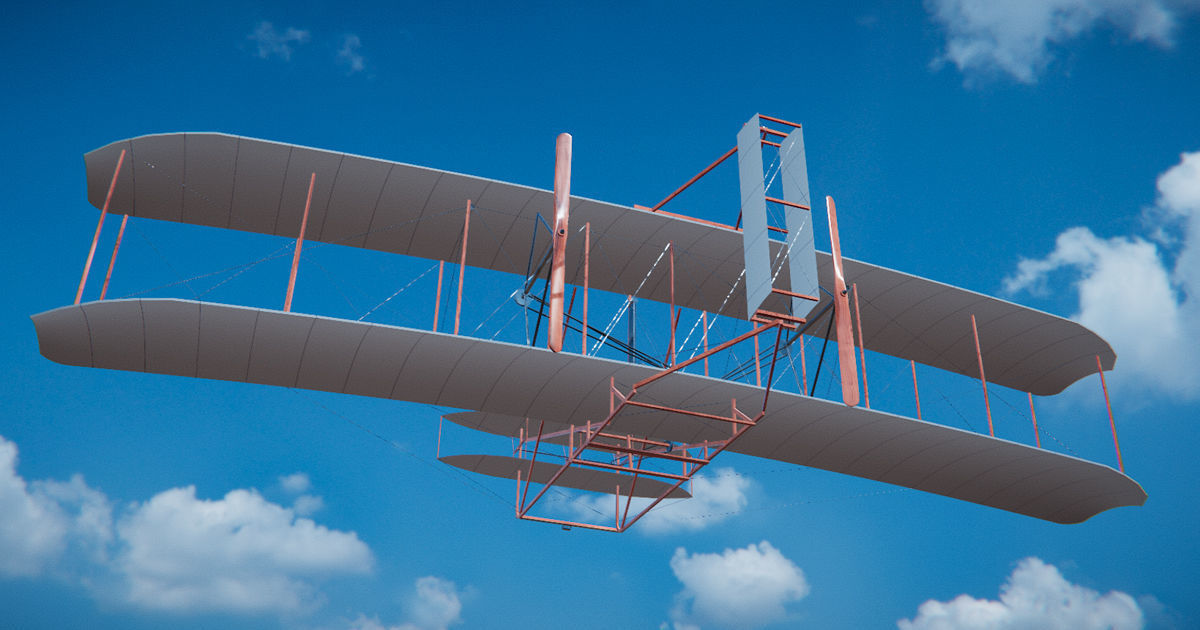
\includegraphics[scale=0.3]{Wright-flyer.jpg}}}
\quad \neq \quad
\vcenter{\hbox{
\includegraphics[scale=0.4]{bird.png}}}
\end{equation}
深度学习是现时\textbf{最强}的学习算法,它可以学习非常复杂的 非线性函数。 问题是怎样利用这件「武器」。 我提出的 architecture 就是 (\ref{eqn:AGI-architecture}),这也是 Richard Sutton 提出的基於 \emp{强化学习} 的模型。 \footnote{AGI 的架构还可以包括 episodic memory 等部分,现在我们考虑的是 minimalist architecture.  如果不用高度抽象的理论,很多时会迷失在支节里。 }

% 为了能控制飞机的方向,Wright brothers 发明了 ``wing warping'' 改变机翼的形状。
时至今日,飞机仍然叫 ``plane'',而这个设计基本上奠定了 100多年以来 飞机的模式。在技术的进化上,这种主导模式的现象称为 dominant design.

我提议 利用 \textbf{逻辑结构},\textbf{约束 $\vect{F}$ 的搜寻空间}(这叫 inductive bias),令它可以更快地学习到人类水平的智能。 这是不是达到 AGI 的最好的方法呢? 不实践是无法知晓的。 Sutton 甚至认为,不需要人为的 bias,纯粹增加\textbf{计算力}就可以了。 
\begin{equation}
\nonumber
\mbox{Richard Sutton (1949-)} \quad \vcenter{\hbox{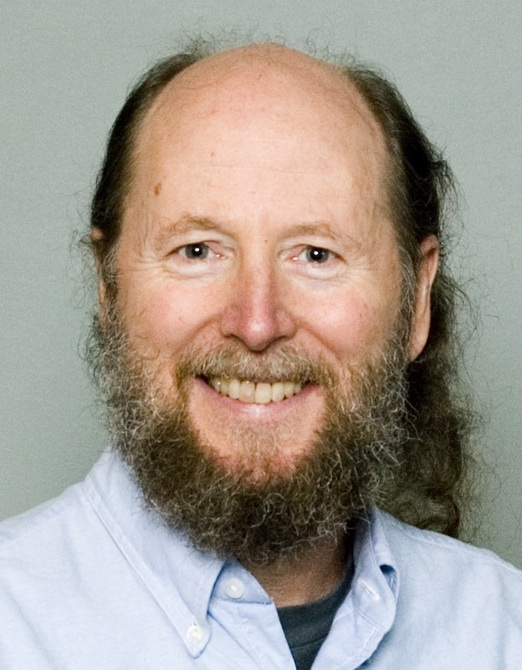
\includegraphics[scale=0.7]{Sutton.jpg}}}
\end{equation}

\section{Associative attention / recommendation of inference}

The word ``attention'' is used here alternatively, not the same as Attention in BERT or Transformers.

It may be advantageous to use a graph neural network (GNN) as the \textbf{state} of our AI system and such that the transition function $F$ maps the current-state GNN to the next-state GNN.

The size of the GNN is the ``working memory'' size and may be moderately large.  So we need an algorithnm to select a subset of nodes in the GNN as \textbf{candidates} for applying deduction:
\begin{equation}
A_1 \wedge A_2 \wedge ... A_n \Rightarrow B .
\end{equation}
There are $M \choose N$ ways of choosing a cluster of $N$ nodes from a total of $M$ nodes.  Finding such subsets is akin to what \textbf{recommendation engines} do, where our problem can be regarded as the recommendation of candidates for logic rules application.

Perhaps an efficient algorithm is to calculate scores of something....

\section*{References}
\cc{欢迎提问和讨论}{Questions, comments welcome} \smiley \\ \vspace*{0.4cm}
% \printbibliography

\end{document}
